\ifx\boi\undefined\ifx\problemname\undefined
\providecommand\sampleinputname{}
\providecommand\sampleoutputname{}
\documentclass[nil]{templates/boi}
\ifdefined\babelprovide
  \babelprovide[import=lv,main]{latvian}
\fi
\problemlanguage{.lv}
\fi
\newcommand{\boi}{Baltijas informātikas olimpiāde}
\newcommand{\practicesession}{Izmēģinājuma kārta}
\newcommand{\contestdates}{27.~aprīlis~-- 1.~maijs, 2018}
\newcommand{\dayone}{1.~diena}
\newcommand{\daytwo}{2.~diena}
\newcommand{\licensingtext}{Šis uzdevums ir licencēts zem CC BY-SA~4.0.}
\newcommand{\problem}{Uzdevums}
\newcommand{\inputsection}{Ievaddati}
\newcommand{\outputsection}{Izvaddati}
\newcommand{\interactivity}{Komunikācija}
\newcommand{\grading}{Testēšana}
\newcommand{\scoring}{Vērtēšana}
\newcommand{\constraints}{Ierobežojumi}
\renewcommand{\sampleinputname}{Ievaddatu paraugs}
\renewcommand{\sampleoutputname}{Izvaddatu paraugs}
\newcommand{\sampleexplanation}[1]{#1.~parauga paskaidrojums}
\newcommand{\sampleexplanations}{Paraugu paskaidrojumi}
\newcommand{\timelimit}{Laika ierobežojums}
\newcommand{\memorylimit}{Atmiņas ierobežojums}
\newcommand{\seconds}{s}
\newcommand{\megabytes}{MB}
\newcommand{\group}{Grupa}
\newcommand{\points}{Punkti}
\newcommand{\limitsname}{Ierobežojumi}
\newcommand{\additionalconstraints}{Papildu ierobežojumi}
\newcommand{\testgroups}{%
Jūsu risinājums tiks testēts uz vairākām testu grupām, par katru no tām var iegūt punktus.
Katra testu grupa satur vienu vai vairākus testus.
Lai iegūtu punktus par testu grupu, jums ir pareizi jāatrisina visi testi šajā grupā.
Jūsu beigu vērtējums par uzdevumu būs starp visiem iesūtījumiem lielākais.%
}
\fi
\def\version{jury-1}
\problemname{Ceļi}
{\em Grafs} ir matemātisks objekts, kas sastāv no {\em virsotnēm} un {\em šķautnēm}, kas katra savieno divas virsotnes. Piemērs grafam ar $4$~virsotnēm un $3$~šķautnēm ir parādīts zemāk.

{\em Ceļš} tiek definēts kā secīga virkne no~$2$ vai vairāk virsotnēm, tāda, ka
starp blakus virsotnēm virknē pastāv šķautne. Šajā uzdevumā mūs interesē tikai
{\em vienkāršie ceļi}, kuros neviena virsotne neparādās vairāk nekā vienu reizi.
Ievērojiet, ka secība ir svarīga; piemēram, ``\texttt{5-6-7}'', ``\texttt{5-7-6}'' un ``\texttt{7-6-5}'' tiek visi uzskatīti par dažādiem ceļiem.

Šajā uzdevumā katra grafa virsotne ir vienā no $K$~krāsām. Uzdevums ir atrast (vienkāršu) ceļu skaitu, kas nesatur virsotnes vienādās krāsās.

\section*{\inputsection}
Pirmā ievada rinda satur trīs veselus skaitļus: $N$ (virsotņu skaits), $M$ (šķautņu skaits) un $K$ (dažādu krāsu skaits).

%($1 \le N, M \le 3 \cdot 10^5, 1 \le K \le 5$).

Otrā ievada rinda satur $N$~skaitļus starp~$1$ un~$K$~--- katras virsotnes krāsu (sākot ar virsotni~$1$ un beidzot ar virsotni~$N$).

Katra no sekojošajām $M$~rindām apraksta šķautni un satur divus veselus skaitļus $a, b$ ($1 \le a, b \le N, a \neq b$)%
~--- divas virsotnes, kuras savieno šķautne. Starp katrām divām virsotnēm būs ne vairāk kā viena šķautne.

\section*{\outputsection}
Izvadiet vienu veselu skaitli~--- ceļu skaitu, kuros visas virsotnes ir dažādās krāsās.
Šis skaitlis vienmēr būs mazāks par~$10^{18}$.

\section*{\constraints}
\testgroups

\noindent
\begin{tabular}{| l | l | l |}
\hline
\group & \points & \limitsname \\ \hline
1      & 23      & $1 \le N, M \le 100, 1 \le K \le 4$ \\ \hline
2      & 20      & $1 \le N, M \le 300\,000, 1 \le K \le 3$ \\ \hline
3      & 27      & $1 \le N, M \le 300\,000, 1 \le K \le 4$ \\ \hline
4      & 30      & $1 \le N, M \le 100\,000, 1 \le K \le 5$ \\ \hline
\end{tabular}

\section*{\sampleexplanation{1}}

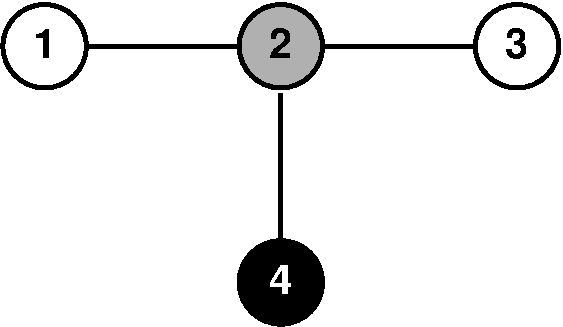
\includegraphics[width=5cm]{pathsfig.pdf}
\nopagebreak

Attēlā parādīts pirmā piemēra grafs, kur katra virsotne ir iezīmēta balta (krāsa~1), pelēka (krāsa~2) vai melna (krāsa~3). Pastāv 10~ceļi, kuros visas virsotnes ir dažādās krāsās: ``\texttt{1-2}'', ``\texttt{2-1}'', ``\texttt{2-3}'', ``\texttt{3-2}'', ``\texttt{2-4}'', ``\texttt{4-2}'', ``\texttt{1-2-4}'', ``\texttt{4-2-1}'', ``\texttt{3-2-4}'' un ``\texttt{4-2-3}''.

Ievērojiet, ka ``\texttt{1}'' neskaitās kā ceļš, jo tā ir viena virsotne, kā arī neskaitās ``\texttt{1-2-3}'', jo tas satur divas virsotnes krāsā~$1$.
